% Created 2013-11-12 Tue 20:00
\documentclass[12pt, a4paper]{article}
\usepackage{polski}
\usepackage[utf8x]{inputenc}
\usepackage[polish]{babel} 
\usepackage{geometry}
\usepackage{hyperref}
\usepackage{amsmath}
\usepackage[numbers]{natbib}
\usepackage{algorithm}
\usepackage{algpseudocode}
\usepackage{float}
\usepackage{graphicx}
\author{Marek Lewandowski, Juliusz Gonera}
\date{}
\title{Porównanie algorytmów znajdowania maksymalnej kliki w grafie}
\begin{document}

\maketitle

\section{Problem maksymalnej kliki}
\label{sec-1}
Kliką nazywamy spójny podgraf, taki że nie jest on zawarty w żadnym innym spójnym podgrafie. Maksymalna klika to klika składająca się z największej liczby wierzchołków. Problem znajdowania maksymalnej kliki w grafie jest problemem NP-zupełnym.

\section{Algorytm}
\label{sec-2}
Do zaimplementowania został wybrany algorytm \ref{basicmc} przechodzący graf w głąb i używający techniki branch-and-bound w celu znalezienia maksymalnej kliki. Algorytm został opisany w \citep{bioinf} (Fig. 2). Zostanie on porównany z dostępną implementacją algorytmu Brona-Kerboscha w bibliotece JGraphT\citep{jgrapht}.

\subsection{Struktury danych}

W algorytmie \ref{basicmc} wykorzystywane są zbiory $Q$ i $Q_{max}$. $Q$ przechowuje wierzchołki aktualnie rozpatrywanej kliki. $Q_{max}$ zawiera wierzchołki największej kliki jaką dotąd udało się znaleźć. $R \subseteq V $ zawiera listę wierzchołków które mogą zostać dodane do $Q$.

\subsection{Opis Algorytmu}

Początkowo $Q := \emptyset, Q_{max} := \emptyset, R := V$. Wybieramy wierzchołek $p$ z dostępnych wierzchołków w $R$ i dodajemy go do $Q$ \algref{basicmc}{addPToQ}. Następnie obliczamy $R_{p} := R \cap \text{adj(}p\text{)}$ który staje się nowym zbiorem wierzchołków do przejrzenia. Procedura EXPAND() jest wywoływana rekursywnie do wyczerpania zbioru wierzchołków $R_{p}$. Jeśli $|Q|+|R| \leq |Q_{max}|$ to $Q \cup R$ może zawierać jedynie klikę niewiększą od $|Q_{max}|$, w tym przypadku algorytm pomija zbędne obliczenia.\algref{basicmc}{skip}

\subsection{Warunek Stopu}

W momencie osiągnięcia $R_{p} = \emptyset$, Zbiór $Q_{max}$ jest maksymalną kliką. Jeśli $|Q| > |Q_{max}|$ zbiór $Q$ zastępuje zbiór $Q_{max}$. Po usunięciu wierzchołka początkowego $p$ z $Q$ i $R$ wybieramy go z wierzchołków pozostałych w $R$ i powtarzamy do przejrzenia wszystkich wierzchołków ($R = \emptyset$)

\subsection{Złożoność Obliczeniowa}
W grafie o $n$ wierzchołkach może być nie więcej niż $3^{\frac{n}{3}}$ maksymalnych klik. Złożoność obliczeniowa algorytmu Brona-Kerboscha wynosi $O(3^{\frac{n}{3}})$.
Jest to także dolne ograniczenie dla złożoności obliczeniowej implementowanego algorytmu. Faktyczne zachowanie algorytmu w zależności od rozmiaru grafu wejściowego zostanie wyznaczone empirycznie.

\subsection{Złożoność pamięciowa}
\label{memory_complexity}

Złożoność pamięciowa implementowanego algorytmu to $O(|V|)$. Ilość pamięci potrzebnej jest wprost proporcjonalna do liczby wierzchołków grafu. Wynika to bezpośrednio z definicji i sposobu użycia zbiorów $Q$, $Q_{max}$ i $R$.

\begin{algorithm}
\caption{BasicMC}\label{basicmc}
\begin{algorithmic}[1]
  
\Procedure{BasicMC}{$V,E$}
\State $Q\gets \emptyset$;
\State $Q_{max}\gets \emptyset$;
\State \Call{EXPAND}{V};
\EndProcedure
\Statex

\Procedure{expand}{$R$}
\While{$R \not= \emptyset$}
  \State $p\gets v\in R$
  \If{$|Q|+|R| > |Q_{max}|$}
    \State $Q \gets Q \cup {p}$\label{addPToQ}
    \State $R_p \gets R \cap adj(p)$
    \If{$R_p \not= \emptyset$}
      \State \Call{EXPAND}{$R_{P}$}
    \ElsIf{$|Q| > |Q_{max}|$}
      \State $Q_{max} \gets Q$
    \EndIf
    \State $Q \gets Q - {p}$
  \Else
    \textbf{ return}\label{skip}
  \EndIf
  \State $R \gets R - p$
\EndWhile
\EndProcedure

\end{algorithmic}
\end{algorithm}

\section{Program}
\label{sec-3}
Program zostanie zaimplementowany w języku Scala. Jest to statycznie typowany język działający na JVM, w pełni kompatybilny z językiem Java.

Program będzie plikiem wykonywalnym wczytującym reprezentację grafu ze standardowego wejścia i wypisującym żądane informacje na standardowe wyjście.

\subsection{Wejście Programu}

Wejściem programu są pliki tekstowe ASCII. Wejście zawiera $|E|+1$ linii nie licząc linii zawierających komentarzy. Pierwsza linijka nie będąca komentarzem jest postaci 
\begin{verbatim}
p col |V| |E|
\end{verbatim}
Gdzie $|V|$ i $|E|$ to odpowiednio liczba węzłów i krawędzi grafu. Następne $|E|$ linijek odpowiada $|E|$ krawędziom grafu. Krawędź $(v, w)$ zapisywana jest jako 
\begin{verbatim}
e W V
\end{verbatim}
i występuje tylko raz. Krawędź $(w, v)$ stanowi części reprezentacji tekstowej grafu. Opisany format jest podzbiorem formatu DIMACS opisanego w \cite{dimacs_format}

\subsection{Opcje Programu}

\subsubsection{Wybór algorytmu}
Program będzie posiadał opcję, która pozwala zmienić algorytm wyszukiwania największej kliki w celu porównania obu algorytmów.

\begin{verbatim}
-j użyj gotowego algorytmu biblioteki JGraph
\end{verbatim}
Przykładowe wywołanie programu:

\begin{verbatim}
./prog < input.txt >> results.txt
./prog -max 600 < input.txt >> results.txt
./prog -j < input.txt >> results.txt
\end{verbatim}

\subsubsection{Ograniczenie czasowe}
Program będzie posiadał opcję, która pozwala określić maksymalny czas działania algorytmu.

\begin{verbatim}
-max N maksymalna liczba sekund na działanie algorytmu
\end{verbatim}
Przykładowe wywołanie programu:

\begin{verbatim}
./prog -max 600 < input.txt >> results.txt
\end{verbatim}

\subsubsection{Ograniczenia na pamięć}
Ograniczenia na pamięć można ustawić z poziomu maszyny wirtualnej Javy korzystając z parametru $-Xmx$

\subsection{Wyjście Programu}

Wyjście programu jest postaci.

\begin{verbatim}
w(g) TIME
\end{verbatim}
Gdzie $\omega(g)$ to rozmiar największej znalezionej kliki a $\text{TIME}$ - czas wykonania algorytmu.

\subsection{Sytuacje awaryjne}
Możliwe sytuacje awaryjne to:

\begin{itemize}
\item zły format wejścia - program będzie zgłaszał błąd, w przypadku wykrycia niewłaściwego formatu wejściowego
\item brak pamięci - błąd obsługiwany przez JVM
\end{itemize}

\section{Projekt testów}
\label{sec-4}

\subsection{Projekt Testów}
Projekt testów został podzielony na 3 części, każda odpowiedzialna za inny aspekt programu.

\subsection{Testy funkcjonane}
Mają na celu pokazanie, że zaimplementowany algorytm jak i reszta aplikacji pozbawiona jest błędów. W ramach tych testów przetestowane zostaną przypadki:

\begin{itemize}
\item grafu pustego z różną liczbą wierzchołków - maksymalna klika powinna wynosić $1$
\item grafu pełnego $K_{n}$ - maksymalna klika wynosi $n$
\item grafu niespójnego zawierającego podgrafy $K_{n_{1}}$ $K_{n_{2}}$ - maksymalna klika wynosi $max(n_{1}, n_{2})$
\item grafu, które jest drzewem - maksymalna klika powinna wynosić $2$
\item kół $W_{n}$ - maksymalna klika powinna wynosić $3$
\end{itemize}

Dla pozostałej części programu - obsługi wejścia, wyjścia, opcji i innych - zostaną wykonane odpowiednie testy.

\subsection{Testy złożoności}
\subsubsection{Złożoność pamięciowa}
Złożoność pamięciowa zostanie ustalona empirycznie na podstawie pomiarów pamięci zużytej przez program dla grafów o różnej wielkości. Oczekiwana złożoność pamięciowa programu to $O(|V|)$ (\ref{memory_complexity}). 

\subsubsection{Złożoność obliczeniowa}
Testy mają na celu empiryczne zmierzenie złożoności obliczeniowej. W tym celu zostaną wygenerowane grafy losowe z różnym prawdopodobieństwem krawędzi i różną liczbą wierzchołków. Dla każdego z wygenerowanych grafów uruchomiony zostanie algorytm. Zebrane wyniki poddane zostaną analizie statystycznej, która pozwoli określić złożoność obliczeniową.



\subsection{Testy porównawcze}
W celu empirycznego porównania wydajności algorytmów zostanie użyty DIMACS Benchmark Set\citep{dimacs}. Jest to zbiór nietrywialnych grafów dla których znana jest liczba wierzchołków tworzących maksymalną klikę w grafie.

Przed faktycznym mierzeniem czasu algorytmu dla danego grafu, algorytm zostanie uruchomiony wielokrotnie dla prostego problemu grafowego w celu ,,nagrzania'' JVM. Sam proces rozgrzewania JVM jest potrzebny do tego, aby program dawał wiarygodne wyniki, które nie są zaburzone optymalizacjami kompilatora JIT, takimi jak generowanie natywnego kodu dla często wykonywanych fragmentów kodu.

\section{Instrukcja obsługi programu}

TODO

\section{Przełożenie algorytmu na kod}
TODO Opis wykorzystania kodu dla programisty (która funkcja co realizuje, w jaki sposób)
TODO algorytm

\section{Porównanie algorytmów}
Algorytmy zostały porównane przy użyciu grafów DIMACS\citep{dimacs}. Są to na tyle nietrywialne grafy, że otrzymanie najlepszego znanego wyniku dla danego grafu zajmuje bardzo długi czas. Najlepszy znany wynik dla grafu C125.9\footnote{graf losowy z 125 wierzchołkami i prawdopodobieństwem krawędzi 0.9}  to $w(g)=34$. Aby ten wynik otrzymać algorytm BasicMQ potrzebował, aż 5 godzin i 25 minut. Klikę o wielkości 33 znalazł po 15 minutach.

Zdecydowaliśmy się zatem ograniczyć czas działania algorytmów do 90 sekund na każdy problem i porównać wyniki pomijając fakt, że są one dużo gorsze od najlepszych rozwiązań.

\subsection{Warunki przeprowadzonych testów na zbiorze DIMACS}
Każdy test został przeprowadzony w następujących warunkach:

\begin{itemize}
\item Program ma do dyspozycji 2G pamięci
\item Czas mierzony jest dopiero od momentu uruchomienia algorytmu, a nie programu\footnote{dla niektórych problemów grafowych, samo zbudowanie grafu trwa parę minut}
\item Algorytm zwraca kolejne coraz lepsze wyniki. Dla każdego wyniku liczony jest czas jego otrzymania.
\item Końcowym wynikiem jest najlepszy wynik otrzymany w ciągu 90 sekund.\footnote{sytuacja, w której algorytm kończy działanie przed upływem czasu jest obsługiwana, ale w praktyce dla grafów ze zbioru DIMACS nie występuje}
\item Algorytm uruchamiany jest bez rozgrzewania JVM. Każde uruchomienie jest na tyle długie, że rozgrzewanie jest zbędne.
\item Program uruchamiany był na procesorze i7 2.6GHz
\end{itemize}

\subsection{Wyniki testów dla grafów ze zbioru DIMACS}
Na początku przyjrzymy się wynikom otrzymanym dla każdego z grafów, a następnie na czas otrzymania tego wyniku. Wyniki przedstawione zostały na wykresach \ref{fig:dimacs-best-part1} i \ref{fig:dimacs-best-part2}. 

\subsubsection{Najlepsze rozwiązania}
Można zauważyć, że dla każdego grafu algorytm BasicMQ daje takie same lub lepsze wyniki przy danych ograniczeniach.

\begin{figure}[H]
  \begin{center}
  \fbox{
    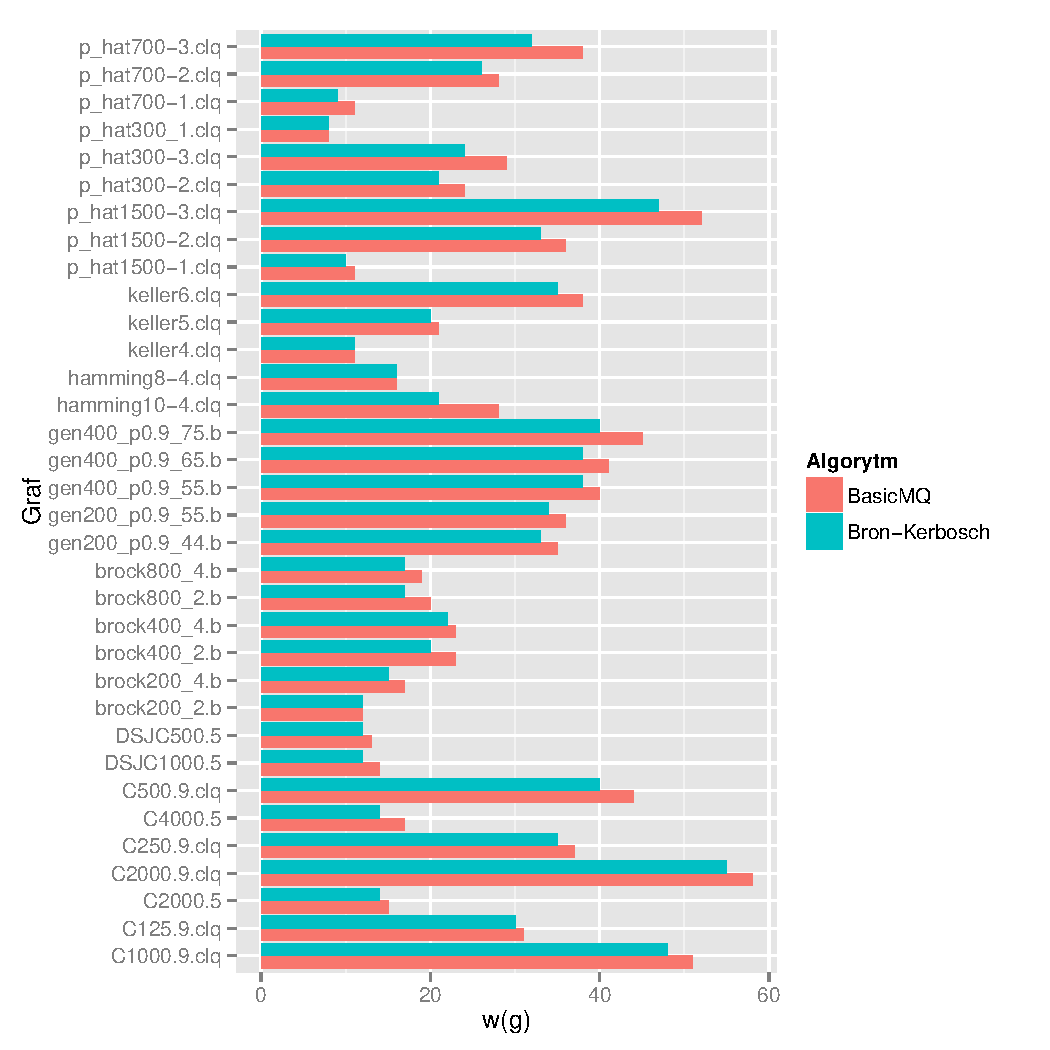
\includegraphics[width=\textwidth]{img/dimacs1.pdf}
  }
  \end{center}
  \caption{Najlepszy wynik dla grafów DIMACS w czasie 90 sekund, część 1}
  \label{fig:dimacs-best-part1}
\end{figure}

\begin{figure}[H]
  \begin{center}
  \fbox{
    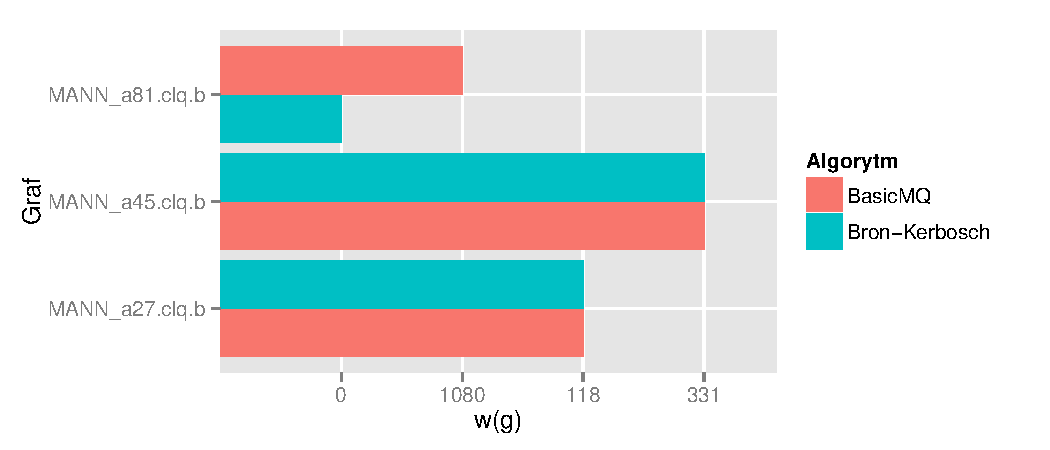
\includegraphics[width=\textwidth]{img/dimacs2.pdf}
  }
  \end{center}
  \caption{Najlepszy wynik dla grafów DIMACS w czasie 90 sekund, część 2}
  \label{fig:dimacs-best-part2}
\end{figure}

Uruchomienie algorytmu dla grafu MANN\_a81.clq dla algorytmu Brona-Kerboscha spowodowało błąd braku pamięci. Graf ten ma 3321 wierzchołków i 5 506 380 krawędzi. Test został uruchomiony ponownie z 4G pamięci. Przy ponownym uruchomieniu algorytm wykonał się poprawnie, ale nie zwrócił żadnych wyników - żadna klika nie została znaleziona w czasie 90 sekund działania algorytmu.

\subsubsection{Czas dla najlepszych rozwiązań}
TODO prawdopodobnie porównywanie czasów dla różnych najlepszych wyników to nie jest najlepsze rozwiązanie, bo gorszy algorytm czyli Bron-Kerbosch pokazuje lepsze czasy ale są to czasy dla gorszych wyników. Trzeba pobawić się trochę R i wybrać odpowiednie wyniki.

Wyniki przedstawione zostały na wykresach \ref{fig:dimacs-best-time-part1} i \ref{fig:dimacs-best-time-part2}. Na wykresie, dla niektórych grafów widzimy bardzo niskie czasy. Nie oznacza to jedak, że algorytm znalazł optymalne rozwiązanie w krótkim czasie. Oznacza to, że algorytm znalazł jedno rozwiązanie dość szybko, a potem nie mógł znaleźć żadnego lepszego rozwiązania w ciągu kolejnych 90 sekund. Dotyczy to grafów 
p\_hat300\_1.clq, p\_hat1500-1.clq, gen200\_p0.9\_44, brock200\_2.b, DSJC500. W niektórych przypadkach dotyczy to tylko algorytmu Brona-Kerboscha np. dla grafu C500.9.clq algorytm BasicMQ znalazł lepsze rozwiązanie przed końcem czasu.



\begin{figure}[H]
  \begin{center}
  \fbox{
    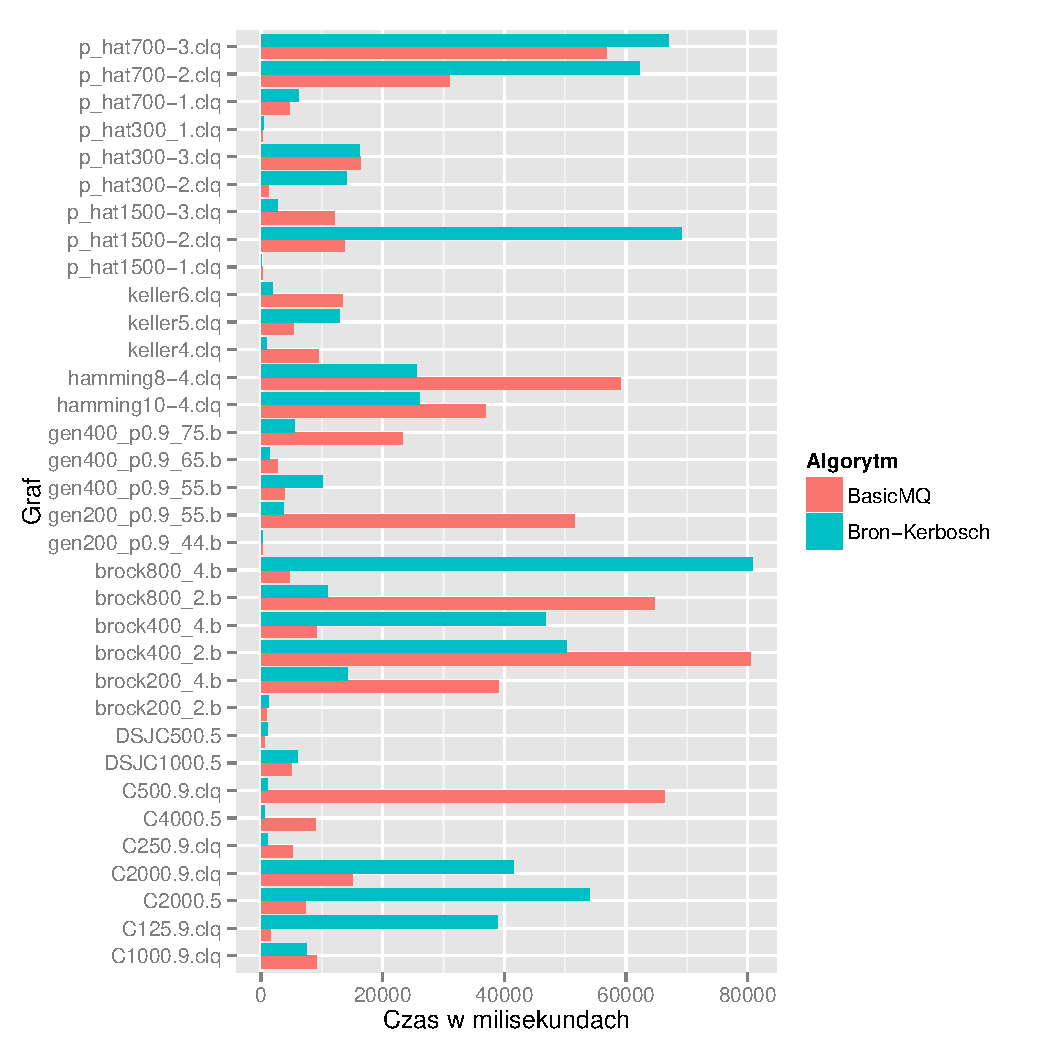
\includegraphics[width=\textwidth]{img/dimacs1czas.pdf}
  }
  \end{center}
  \caption{Czas osiągnięcia wyniku dla grafów DIMACS w czasie 90 sekund, część 1}
  \label{fig:dimacs-best-time-part1}
\end{figure}

\begin{figure}[H]
  \begin{center}
  \fbox{
    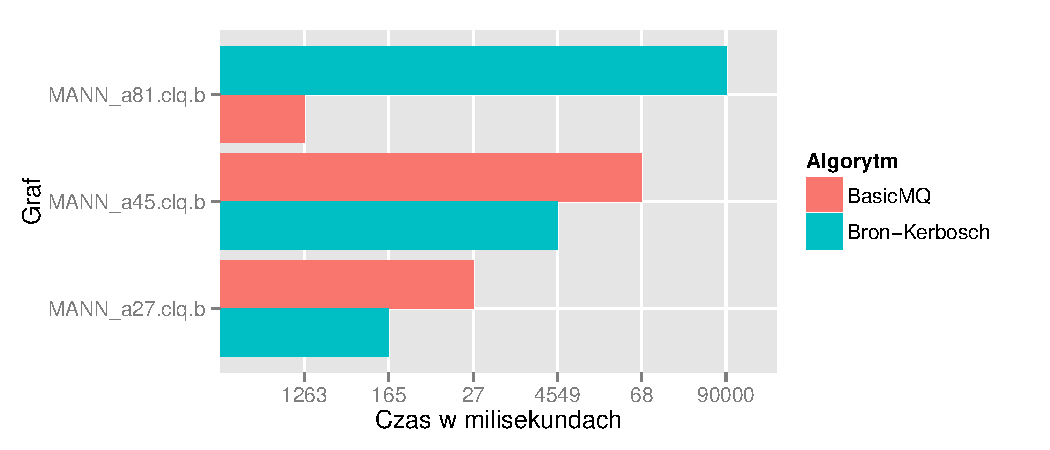
\includegraphics[width=\textwidth]{img/dimacs2czas.pdf}
  }
  \end{center}
  \caption{Czas osiągnięcia wyniku dla grafów DIMACS w czasie 90 sekund, część 2}
  \label{fig:dimacs-best-time-part2}
\end{figure}


\subsection{Szybkość znajdowania kolejnych rozwiązań}
Test ten został przeprowadzony na grafie C125.9 z ograniczeniem 20 minut. Pozostałe warunki testowe są takie same. Program uruchomiony został z opcją wyświetlania coraz lepszych wyników. Wykres \ref{fig:ProgressC125.9-20min} przedstawia wyniki tego testu. Można zauważyć kilka ciekawych rzeczy. Po pierwsze algorytm BasicMQ zdążył znaleźć lepszy wynik. Najlepszy wynik znaleziony przez algorytm Brona-Kerboscha został znaleziony przez algorytm BasicMQ w czasie o rząd wielkości mniejszym. Widać tutaj także regularność - BasicMQ znajduje rozwiązania szybciej od algorytmu Brona-Kerboscha dla tego typu grafu.

\begin{figure}[H]
  \begin{center}
  \fbox{
    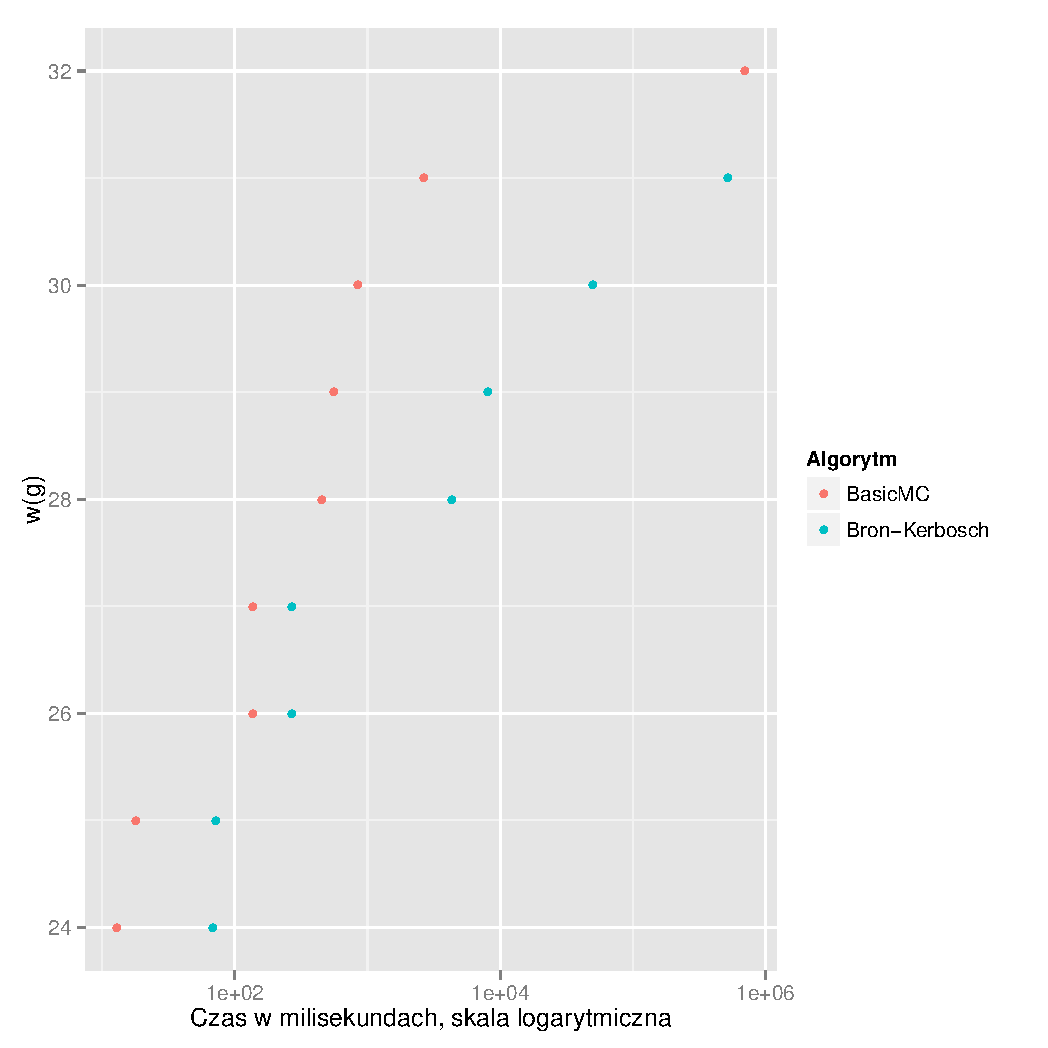
\includegraphics[width=\textwidth]{img/progress.pdf}
  }
  \end{center}
  \caption{Kolejne wyniki w czasie dla grafu C125.9 z ograniczeniem 20 minut}
  \label{fig:ProgressC125.9-20min}
\end{figure}

\section{Badanie złożoności}

TODO

\section{Testy kodu TODO lepsza nazwa}

TODO pokazać, że to co napisaliśmy, że będziemy testować zostało przetestowane i działa. Screen z uruchomienia sbt test?


\nocite{*}
\bibliographystyle{plainnat}
\bibliography{bibliography}
\end{document}
